\documentclass[12pt, a4paper]{article}
\usepackage[utf8]{inputenc}
\usepackage{listings}
\usepackage{courier}
\usepackage{fancyhdr}
\usepackage{color}
\usepackage{xcolor}
\usepackage{caption}
\usepackage{graphicx}
\usepackage{url}
\usepackage[titletoc]{appendix}
\usepackage{textcomp}
\usepackage{pdfpages}
\usepackage[colorlinks]{hyperref}
\hypersetup{urlcolor=blue}


\definecolor{light-gray}{gray}{0.95}

\lstset{
 upquote=true,
 showspaces=false,
 showtabs=false,
 frame=none,
 tabsize=2,
 breaklines=true,
 numbers=none,
 showstringspaces=false,
 breakatwhitespace=true,
 escapeinside={(*@}{@*)},
 keywordstyle=\bfseries,
 basicstyle=\footnotesize\ttfamily,
}

\newcommand{\code}[1]{{\footnotesize\texttt{#1}}}

\setlength\parindent{0pt} % Indentazione paragrafi
\setlength{\parskip}{1ex plus 0.5ex minus 0.2ex} % Spaziatura paragrafi


\title{SDN controller clustering \\ \large Computer Networks module - SDN assignment}
\author{Michele Zanotti}
\date{Spring term 2018}

\pagestyle{fancy}
\fancyhf{}
\lhead{Computer Networks}
\rhead{SDN assignment}
\rfoot{\thepage}

\begin{document}

\maketitle
\begin{figure}[htb]
	\centering
	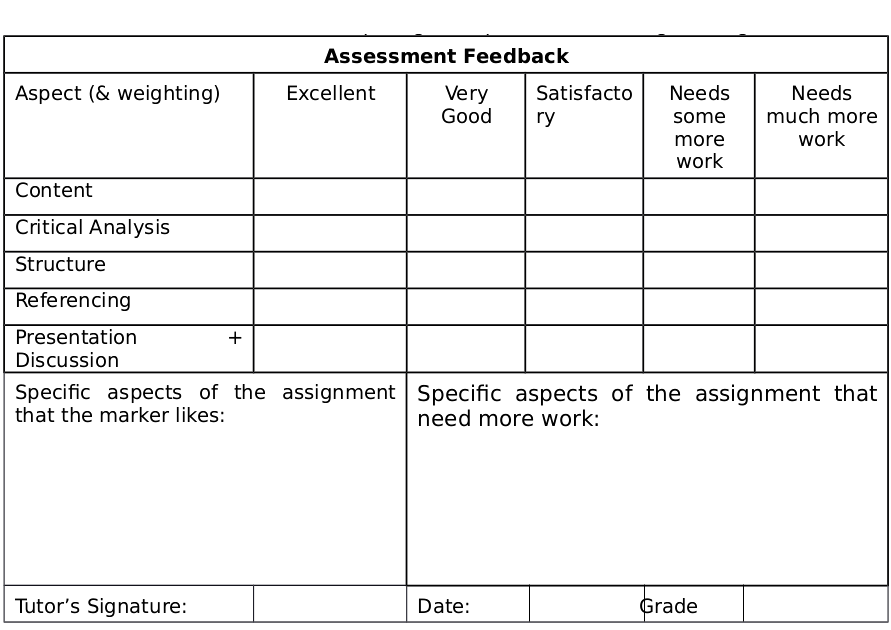
\includegraphics[width=1\linewidth]{img/valuation-table.png}
\end{figure}

\newpage





\section*{Overview}
In this paper are proposed four different lab activities meant to teach how to implement
a cluster of controllers inside Mininet using some of the most common available methods.
Each activity focuses on a single method and uses it to implement a given topology.

In particular, in each activity the following methods will be explained:
\begin{itemize}
  \item \textbf{Activity 1}: implement a network with multiple controllers using a python
  script and the middle-level Mininet API
  \item \textbf{Activity 2}: implement a network with multiple local controllers using a python
  script, a custom switch class and the topology classes provided by the Mininet high-level API
  \item \textbf{Activity 3}: how to dynamically connect the switches of a Mininet
  network to different controllers using the tool ovs-vsctl.
\end{itemize}

The paper also includes a fourth lab activity (\textbf{Activity 4}), which is a conclusive challenge meant
to let the reader test the knowledge acquired with the execution of the previous
four activities. Each activity moreover contains some final questions aimed to make the reader
reflect about what he did during that specific activity and possibly make him try to
bring minor changes to the implemented topology. The solution for the activity 4
and the answers for the questions included in the previous activities can be
found in appendix A.

It's important to point out that all the proposed activities are meant to be
only an introduction to SDN controller clustering, therefore this paper won't cover
some of the aspects that have to be considered when implementing a cluster of
controllers in a real-world context, such as load balancing and communication
between controllers. More information about these topics can be found in references
\cite{ref-2}, \cite{ref-1} and \cite{ref-9}.
The communication between different controllers can however be automatically managed
by Mininet, the network emulator used in these paper activities. When in fact a
network with multiple local controllers is implemented inside the emulator, all
the local controllers are executed inside the kernel space on a single machine
and therefore they can communicate with each other without an external
communication mechanism being necessary.

\section*{Lab activity 1}





\subsection*{Learning objectives}
After finishing this lab activity you will be able to:
\begin{itemize}
  \item Implement a cluster of local controller inside Mininet using the python
  middle-level Mininet API
  \item Test the network connectivity and the performance of a network which
  includes a cluster of local controllers
  \item Understand the main functions provided by the middle-level Mininet API required
  to implement a cluster of local controllers
\end{itemize}






\subsection*{Scenario}
In this activity you will implement the simple topology shown in figure *** using
a Python script and the middle-level API provided by Mininet. The two controllers
showned in the topology diagram will be local controllers for this activity.
The topology has two different switches: each one will be connected to a different
local controller.

Begin by creating a new Python script, then import Mininet classes required for
this activity and define the function that will be used to create the topology.
Inside the body of this function, create a new Mininet netowrk and add to it the
required hosts, switches, links and controllers. After writing the script, execute
it to create the network and test its connectivity and performance.

This lab activity assumes you are proficient in [...]. A basic knowledge of the
Python programming language is also assumed.





\subsection*{Task 1: write the skeleton of the Python script}
\subsubsection*{Step 1}
Create a new python script and edit with the text editor you prefer. If your editing
it inside the Mininet virtual machine, it is suggested to use Vim text editor.

\subsubsection*{Step 2}
Import the Python classes from the Mininet API:
\begin{lstlisting}
#!/usr/bin/python
from mininet.net import Mininet
from mininet.node import Controller, OVSSwitch
from mininet.cli import CLI
from mininet.log import setLogLevel, info
\end{lstlisting}

\subsubsection*{Step 3}
Make the script executable onyl as a program, set the log level to ``info''
and call the function \code{multiControllerNet()}, which will be defined in the next
step:
\begin{lstlisting}
if __name__ == '__main__':
    setLogLevel( 'info' )
    multiControllerNet()
\end{lstlisting}

\subsubsection*{Step 4}
Define the function that will be used to create the topology:
\begin{lstlisting}
def multiControllerNet():
\end{lstlisting}

\subsubsection*{Step 6}
Inside the body of the function \code{multiControllerNet()} create a new Mininet
network:
\begin{lstlisting}
net = Mininet( controller=Controller, switch=OVSSwitch )
\end{lstlisting}

The Mininet network is created invoking the Mininet constructor: the parameters
passed to the constructor are the Controller class and the OVSSwitch class, therefore
the Stanford/OpenFlow reference controllers and Open vSwitch switches will be used
in the network we are goind to create. Note that these two classes are
the default parameters in the Mininet constructor, so it is not really necessary
to specify them.

\subsubsection*{Step 7}
Save the text file as ``\emph{controllers-1.py}'' in your custom directory inside
the mininet virtual machine.





\subsection*{Task 2: add hosts to the network}
\subsubsection*{Step 1}
Inside the body of the function \code{multiControllerNet()} add the following line
of code in order to print to the console that hosts are being created:
\begin{lstlisting}
info( "*** Creating hosts \n" )
\end{lstlisting}

\subsubsection*{Step 2}
Still inside the body of the function \code{multiControllerNet()}, create the
four hosts required for the topology by adding them to the mininet network
previously created:
\begin{lstlisting}
h1 = net.addHost('h3')
h2 = net.addHost('h4')
h3 = net.addHost('h5')
h4 = net.addHost('h6')
\end{lstlisting}
The function used to add the hosts to the network is \code{addHost('name')}, which
accept as parameter the name of the host that will be created. The hosts names in
this network therefore will we \code{h3}, \code{h4}, \code{h5} and \code{h6}.





\subsection*{Task 3: add switches to the network}
\subsubsection*{Step 1}
Inside the body of the function \code{multiControllerNet()} add the following line
of code in order to print to the console that switches are being created:
\begin{lstlisting}
info( "*** Creating switches \n" )
\end{lstlisting}

\subsubsection*{Step 2}
Still inside the body of the function \code{multiControllerNet()}, create the
two switches required for the topology by adding them to the mininet network
previously created:
\begin{lstlisting}
s1 = net.addSwitch('s1')
s2 = net.addSwitch('s2')
\end{lstlisting}







\subsection*{Task 4: create links between nodes}
\subsubsection*{Step 1}
Inside the body of the function \code{multiControllerNet()} add the following line
of code in order to print to the console that links are being created:
\begin{lstlisting}
info( "*** Creating links \n" )
\end{lstlisting}

\subsubsection*{Step 2}
Still inside the body of the function \code{multiControllerNet()}, create four
links between the hosts and the switches and the link between the two switches:
\begin{lstlisting}
net.addLink( h3, s1 )
net.addLink( h4, s1 )
net.addLink( h5, s2 )
net.addLink( h6, s2 )
net.addLink( s1, s2 )
\end{lstlisting}








\subsection*{Step 5: create controllers} \label{sec:step-5}
In this step we are going to create two local SDN controllers. The code we have to
add to the script is the following:

\code{info( "*** Creating (reference) controllers\textbackslash n" )} \\
\code{c1 = net.addController( 'c1', port=6633 )} \\
\code{c2 = net.addController( 'c2', port=6634 )}

Note that we specified a different TCP port for each controller (the controllers
will listen on the specified port for switches that want to set up a connection).

\textbf{Why did we specify a different port for each controller?}

\hrulefill

\hrulefill
% Because each swtich has to setup one TCP connection to each controller and
% it's not possible having more than one TCP connection on the same port, so
% specifying two different ports makes it possible to connect one single switch
% to multiple controllers.


\subsection*{Step 6: start the network}
After adding all the required nodes to the network we can finally start it. In order
to do that, we have to build the mininet network and start the controllers and the
switches:

\code{info( "*** Starting network\textbackslash n" )} \\
\code{net.build()} \\
\code{c1.start()} \\
\code{c2.start()} \\
\code{s1.start( [ c1 ] )} \\
\code{s2.start( [ c2 ] )}

In the last two lines of code we used the function start() to start the two switches,
passing as parameter

After this step, the python script required to build the topology for the task one
is completed. The full script is shown in listing \ref{lst:task-1-complete-script}.



\subsection{Step 7: test network connectivity and performance}
The final step is execute the script and test the created topology: try to verify
the network connectivity between all hosts and the bandwidth between \code{h3} and \code{h6}.
Write in the lines below the commands you used and the results you obtained.

\hrulefill

\hrulefill

\hrulefill

\begin{lstlisting}[label=lst:task-1-complete-script, caption=Task 1 complete python script]
#!/usr/bin/python
from mininet.net import Mininet
from mininet.node import Controller, OVSSwitch
from mininet.cli import CLI
from mininet.log import setLogLevel, info

def multiControllerNet():
    net = Mininet( controller=Controller, switch=OVSSwitch )

    info( "*** Creating hosts\n" )
    h1 = net.addHost('h3')
    h2 = net.addHost('h4')
    h3 = net.addHost('h5')
    h4 = net.addHost('h6')

    info( "*** Creating switches\n" )
    s1 = net.addSwitch( 's1' )
    s2 = net.addSwitch( 's2' )

    info( "*** Creating links\n" )
    net.addLink( h3, s1 )
    net.addLink( h4, s1 )
    net.addLink( h5, s2 )
    net.addLink( h6, s2 )
    net.addLink( s1, s2 )

    info( "*** Creating (reference) controllers\n" )
    c1 = net.addController( 'c1', port=6633 )
    c2 = net.addController( 'c2', port=6634 )

    info( "*** Starting network\n" )
    net.build()
    c1.start()
    c2.start()
    s1.start( [ c1 ] )
    s2.start( [ c2 ] )

    info( "*** Running CLI\n" )
    CLI( net )

    info( "*** Stopping network\n" )
    net.stop()

if __name__ == '__main__':
    setLogLevel( 'info' )  # for CLI output
    multiControllerNet()
\end{lstlisting}

\lstset{
 upquote=true,
 showspaces=false,
 showtabs=false,
 frame=none,
 tabsize=2,
 breaklines=true,
 numbers=none,
 showstringspaces=false,
 breakatwhitespace=true,
 escapeinside={(*@}{@*)},
 keywordstyle=\bfseries,
 basicstyle=\footnotesize\ttfamily,
}

\section*{Lab activity 2}

\subsection*{Topology diagram}
\begin{figure}[htb]
	\centering
	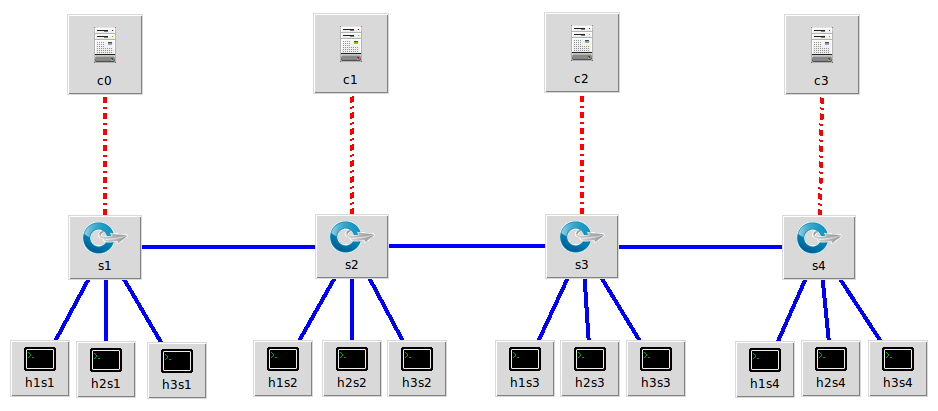
\includegraphics[width=1\linewidth]{img/topology-2.png}
	\caption{the topology that will be implemented during this lab activity.
  It is a linear topology with four switches connected to each other,
  each one connected to three hosts. Each switch is linked to a different
  SDN controller. All the controllers can be assumed local.}
	\label{fig:topology-2}
\end{figure}

\subsection*{Learning objectives}
After finishing this lab activity you will be able to:
\begin{itemize}
  \item create a custom switch class that extends the OVSSwitch class provided
  by the Mininet Python API
  \item implement a cluster of local/remote controllers inside Mininet using a custom
  switch class and the topology classes provided by the Mininet high-level API
  \item implement more complex topologies with multiple controllers using a
  few lines of Python code
  \item reflect upon the method used in this activity for implementing a cluster of controllers
  and compare it with the method shown in Activity 1, focusing on the advantages
  and disadvantages of each method
  \item test the network connectivity and the performance of a network with multiple
  controllers.
\end{itemize}






\subsection*{Scenario}
In this activity you will implement the topology shown in figure \ref{fig:topology-2} using
a Python script and the classes provided by the high-level Mininet API, which
represent topology templates. In order to use these classes for creating a network
with multiple controllers, you will have to define a new switch class that extends
the standard OVSSwitch class provided by the API.

Begin by creating a new Python script and importing the required Mininet classes.
Create the controllers shown in the topology diagram and define
a custom switch class which extends the class \code{OVSSwitch}. Define a function for creating
the network and inside its body use one of the topology templates provided
by the API to implement the required topology.
After writing the script, execute it and test the network connectivity and its
performance. To conclude, answer the questions proposed in the last task.

This lab activity assumes that:
\begin{itemize}
  \item you are proficient in SDN networks
  \item you are proficient in Mininet network emulator
  \item you have a basic knowledge of Python object-oriented
  \item you have already completed Activity 1.
\end{itemize}

The activity is inspired by the script \textit{controllers.py} \parencite{ref-6} included in the
examples provided by Mininet, which can therefore be used as
an additional example of how a topology with multiple controllers can be implemented
inside Mininet using a Python script and defining a custom switch class.





\subsection*{Task 1: create the controllers}
\subsubsection*{Step 1}
Create a new Python script and edit it with the text editor you prefer. If you're editing
it inside the Mininet virtual machine, it is suggested to use Vim text editor.

\subsubsection*{Step 2}
Import the required Python classes from the Mininet API:
\begin{lstlisting}
#!/usr/bin/Python
from mininet.net import Mininet
from mininet.node import OVSSwitch, Controller
from mininet.topo import LinearTopo
from mininet.log import setLogLevel
from mininet.cli import CLI
\end{lstlisting}

\subsubsection*{Step 3}
Create the four required controllers, specifying for each one a different name and
a different TCP port:
\begin{lstlisting}
c0 = Controller( 'c0', port=6633 )
c1 = Controller( 'c1', port=6634 )
c2 = Controller( 'c2', port=6635 )
c3 = Controller( 'c3', port=6636 )
\end{lstlisting}

\subsubsection*{Step 4}
Create a new array and initialize it with the four created controllers:
\begin{lstlisting}
controllers = [c0, c1, c2, c3]
\end{lstlisting}
This array will be used later in the script to easily add all the controllers
to the network using a for loop (see Step 4 of Task 3).

\subsubsection*{Step 5}
Create a map that associates each switch to the relative controller:
\begin{lstlisting}
cmap = { 's1': c0, 's2': c1, 's3': c2, 's4' : c3 }
\end{lstlisting}






\subsection*{Task 2: create a custom switch class}
\subsubsection*{Step 1}
Define a new class called \code{MultiSwitch} wich extends the class
\code{OVSSwitch} provided by the Mininet API:
\begin{lstlisting}
class MultiSwitch( OVSSwitch ):
\end{lstlisting}

\subsubsection*{Step 2}
Overwrite the method \code{start} of the superclass \code{OVSSwitch}:
\begin{lstlisting}
def start( self, controllers ):
  return OVSSwitch.start( self, [ cmap[ self.name ] ] )
\end{lstlisting}
The method simply returns the result of the call to the method \code{start} of the
superclass passing as parameter the controller associated to the switch name, as defined by
the map \code{cmap} previously created. In this way each switch will connect to
the relative controller according to the map \code{cmap}.






\subsection*{Task 3: define a function that creates the topology}
\subsubsection*{Step 1}
Define a new function called ``multiControllerNet'':
\begin{lstlisting}
def multiControllerNet():
\end{lstlisting}

\subsubsection*{Step 2}
Create a new linear topology using the class \code{LinearTopo} provided by
the API, specifying as parameters the number of switches \code{k} and the
number of hosts per switch \code{n}:
\begin{lstlisting}
topo = LinearTopo( k=4, n=3 )
\end{lstlisting}

\subsubsection*{Step 3}
Create a new Mininet network, specifying as constructor parameters the topology
called \code{topo} created in the previous step, the class \code{MultiSwitch}
defined in task 2 and the value \code{build=False} for preventing Minined to build
the network immediately:
\begin{lstlisting}
net = Mininet( topo=topo, switch=MultiSwitch, build=False)
\end{lstlisting}

\subsubsection*{Step 4}
Add the controllers to the network:
\begin{lstlisting}
for c in controllers:
  net.addController(c)
\end{lstlisting}

\subsubsection*{Step 5}
Build the network and start it:
\begin{lstlisting}
net.build()
net.start()
\end{lstlisting}

\subsubsection*{Step 6}
Start the CLI and stop the network:
\begin{lstlisting}
CLI( net )
net.stop()
\end{lstlisting}




\subsection*{Task 4: finalize the script and save it}
\subsubsection*{Step 1}
Make the script executable only as a program and set the CLI verbosity level
to ``info'':
\begin{lstlisting}
if __name__ == '__main__':
    setLogLevel( 'info' )
    multiControllerNet()
\end{lstlisting}

\subsubsection*{Step 2}
Save the text file as ``\emph{activity-2.py}'' in your custom directory inside
the mininet virtual machine.






\subsection*{Task 5: execute the script and test the network}
After finishing the task 4 the script for implementing the required topology is
completed. The full script is shown in listing \ref{lst:activity-2-script} at the
bottom of this activity.

\subsubsection*{Step 1}
Execute the script as root: \\
\code{\$ sudo python activity-2.py}

\subsubsection*{Step 2}
Test the created topology: verify the network connectivity between all hosts.
Write in the lines below the commands you used and the results you obtained.

\hrulefill

\hrulefill

\hrulefill

\hrulefill

\subsubsection*{Step 3}
Verify the bandwidth and the delay between the hosts \code{h1s1} and \code{h3s4}.
Write in the lines below the commands you used and the results you obtained.

\hrulefill

\hrulefill

\hrulefill

\hrulefill





\subsection*{Task 6: reflection}
\subsubsection*{1 - In this activity you implemented a network with multiple
controllers using a custom switch class and the high-level API. Which are
the advantages of using this method insted of the one used in Activity 1? What
about the disadvantages?}
\hrulefill

\hrulefill

\hrulefill

\hrulefill


\subsubsection*{2 - In this activity the topology shown in figure \ref{fig:topology-2}
was implemented assuming that all the controllers were local controllers. How would
you have to change the Python script you created in this activity in order
to use remote controllers instead of local ones?}
\hrulefill

\hrulefill

\hrulefill

\hrulefill


\subsubsection*{3 - Try to modify the script you realized in order to have only
two controllers instead of four, each one linked to two different switches. Each
switch must be linked to a controller. }
\hrulefill

\hrulefill

\hrulefill

\hrulefill






\lstset{
 upquote=true,
 showspaces=false,
 showtabs=false,
 frame=single,
 tabsize=2,
 breaklines=true,
 numbers=left,
 showstringspaces=false,
 breakatwhitespace=true,
 escapeinside={(*@}{@*)},
 keywordstyle=\bfseries,
 basicstyle=\scriptsize\ttfamily,
}

\begin{minipage}{\linewidth}
\begin{lstlisting}[label=lst:activity-2-script, caption=the complete Python script required for Activity 2]
#!/usr/bin/Python
from mininet.net import Mininet
from mininet.node import OVSSwitch, Controller
from mininet.topo import LinearTopo
from mininet.log import setLogLevel
from mininet.cli import CLI

c0 = Controller( 'c0', port=6633 )
c1 = Controller( 'c1', port=6634 )
c2 = Controller( 'c2', port=6635 )
c3 = Controller( 'c3', port=6636 )

controllers = [c0, c1, c2, c3]
cmap = { 's1': c0, 's2': c1, 's3': c2, 's4' : c3 }


class MultiSwitch( OVSSwitch ):
  def start( self, controllers ):
    return OVSSwitch.start( self, [ cmap[ self.name ] ] )


def multiControllerNet():
  topo = LinearTopo( k=4, n=3 )
  net = Mininet( topo=topo, switch=MultiSwitch, build=False)

  for c in controllers:
    net.addController(c)

  net.build()
  net.start()
  CLI( net )
  net.stop()

if __name__ == '__main__':
  setLogLevel( 'info' )
  multiControllerNet()
\end{lstlisting}
\end{minipage}

\lstset{
 upquote=true,
 showspaces=false,
 showtabs=false,
 frame=none,
 tabsize=2,
 breaklines=true,
 numbers=none,
 showstringspaces=false,
 breakatwhitespace=true,
 escapeinside={(*@}{@*)},
 keywordstyle=\bfseries,
 basicstyle=\footnotesize\ttfamily,
}






\section*{Lab activity 3}
\subsection*{Topology diagram}
\begin{figure}[htb]
	\centering
	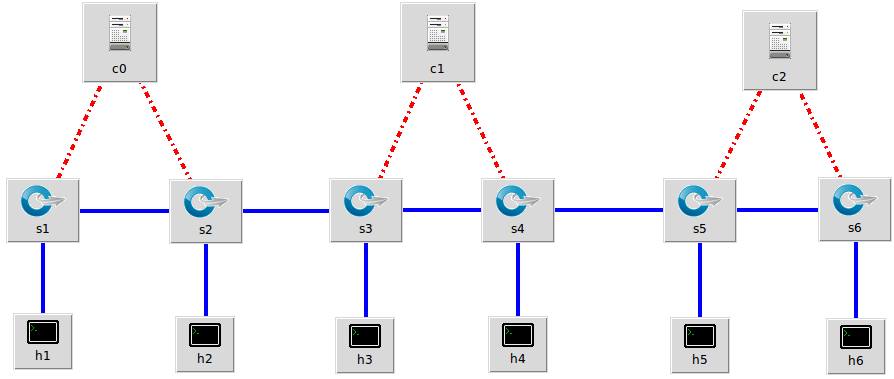
\includegraphics[width=1\linewidth]{img/topology-3.png}
	\caption{the simple linear topology that will be implemented in this activity. It is
  assumed that c1 and c2 are remote controllers running on the same machine
  on which Mininet is running, respectively on the TCP ports 6634 and 6635,
  while c0 is a local controller.}
	\label{fig:topology-3}
\end{figure}







\subsection*{Learning objectives}
After finishing this lab activity you will be able to:
\begin{itemize}
  \item use the tool ovs-vsctl for implementing a cluster of controllers inside Mininet
  \item test the network connectivity and the performance of a network with multiple
  controllers
  \item dynamically set the controller for any switch of a generic running Mininet
  network using the tool ovs-vsctl.
\end{itemize}






\subsection*{Scenario}
In this activity you will implement the topology shown in figure \ref{fig:topology-3}
using the command \code{mn} to create and start a new Mininet network, passing
\code{--topo} as parameter to specify the required topology. You will then
use the tool ovs-vsctl in order to set the controller for each switch according
to the topology diagram shown in figure \ref{fig:topology-3}.

Begin by creating and starting a new Mininet network using the command \code{mn}.
Once the network is running, start the remote controllers and use the tool ovs-vsctl
for setting the controller for each switch according to the topology diagram.
To conclude, test the network verifying the connectivity between all hosts.

This lab activity assumes that:
\begin{itemize}
  \item you are proficient in SDN networks
  \item you are proficient in Mininet network emulator
  \item you have already completed the previous lab activities of this paper.
\end{itemize}






\subsection*{Task 1: create and start the network}
Create and start a new Mininet network, using the parameter \code{--topo} to
specify the required topology:
\begin{lstlisting}
$ sudo mn --topo linear,6
\end{lstlisting}
After executing this command the network will be running and a single local controller
(called \code{c0}) will be used for all the switches.


\subsection*{Task 2: start the remote controllers}
\subsubsection*{Step 1}
Open a new terminal and move to the directory \code{/home/mininet/pox}

\subsubsection*{Step 2}
Start the first POX controller, using the component \code{forwarding.l2\_learning}
for making the OpenFlow switches act as L2 learning switches and the component
\code{openflow.of\_01} for specifying the TCP port to listen for connections on.

\lstset{basicstyle=\scriptsize\ttfamily}
\begin{lstlisting}
$ sudo ./pox.py forwarding.l2_learning openflow.of_01 --port=6634
\end{lstlisting}

\subsubsection*{Step 3}
Open a new terminal and repeat step 1 and step 2 for starting the second controller.
Remember to specify the correct TCP port, which this time will be 6635 instead of 6634.




\subsection*{Task 3: set the controller for each switch}
\subsubsection*{Step 1}
Open a new terminal and use ovs-vsctl to connect the switch \code{s3} to the POX
controller listening on port 6634 \parencite{ref-8}:
\begin{lstlisting}
$ sudo ovs-vsctl set-controller s3 tcp:127.0.0.1:6634
\end{lstlisting}
On the terminal with which you started that controller you should see that a new
switch has connected, like in the screenshoot below:
\begin{figure}[htb]
	\centering
	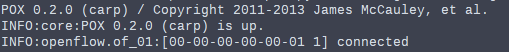
\includegraphics[width=1\linewidth]{img/controller-connection.png}
\end{figure}


\subsubsection*{Step 2}
Use ovs-vsctl to connect the switch \code{s4} to the POX controller listening on
port 6634:
\begin{lstlisting}
$ sudo ovs-vsctl set-controller s4 tcp:127.0.0.1:6634
\end{lstlisting}
Again, on the controller's terminal you should se that the switch has connected
to the controller.


\subsubsection*{Step 3}
Apply the same proceeding showed in the first two step to connect the switches
\code{s5} and \code{s6} to the POX controller listening on port 6635.



\subsection*{Task 4: test the network}
Test the connectivity between all hosts.

\section*{Lab activity 4: final challenge}

\subsection*{Topology diagram}
\begin{figure}[htb]
	\centering
	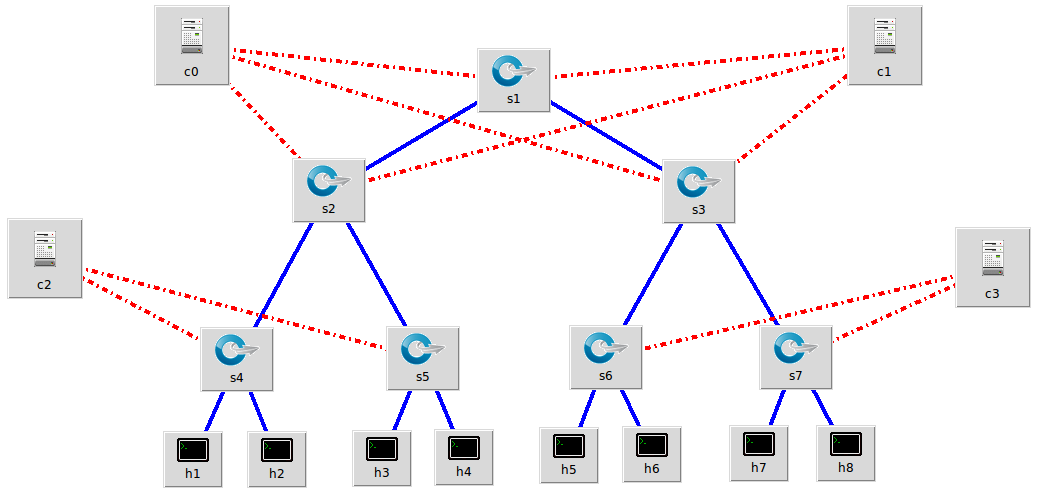
\includegraphics[width=1\linewidth]{img/challange-topology.png}
	\caption{the topology that you will have to implement in this activity, or rather
  a tree topology with multiple SDN controllers.
  The controllers \code{c2} and \code{c3} are local while \code{c0} and \code{c1}
  are remote controllers running on the same machine on which Mininet is running,
	listening respectively on TCP ports 6635 and 6636.}
	\label{fig:challenge-topology}
\end{figure}




\subsection*{Learning objectives}
After finishing this lab activity you will be able to apply what you have learnt
through the previous lab activities in order to implement on your own a given
topology which includes multiple controllers.





\subsection*{Scenario}
In this activity you will have to implement on your own the topology shown in
figure \ref{fig:challenge-topology} using the method you think is most appropriate
among those previously shown in this paper.

The activity is meant to let you test the knowledge you acquired through the
previous three activities proposed in this paper, therefore it assumes that you
have already completed them successfully.

The solution for this activity is available in the appendix A of this paper.



\subsection*{Task 1: implement the topology}
Implement the topology shown in figure \ref{fig:challenge-topology} using the method
you think is most appropriate.

\subsection*{Task 2: fix the network}
Assume that the controller \code{c3} failed and it's not working anymore: without
shutting down the whole network, fix the problem by connecting the switches served by \code{c3}
to the other available remote controller.

\section*{Appendix A}
\lstset{
 upquote=true,
 showspaces=false,
 showtabs=false,
 frame=none,
 tabsize=2,
 breaklines=true,
 numbers=none,
 showstringspaces=false,
 breakatwhitespace=true,
 escapeinside={(*@}{@*)},
 keywordstyle=\bfseries,
 basicstyle=\scriptsize\ttfamily,
 moredelim=**[is][\color{red}]{@}{@},
}

In this appendix are reported the answers to the questions proposed in all the
previous lab activities.


\subsection*{Activity 1}

\subsubsection*{Task 7 - Step 2}
\textit{Test the created topology: verify the network connectivity between all hosts.
Write in the lines below the commands you used and the results you obtained.}
\begin{figure}[htb]
	\centering
	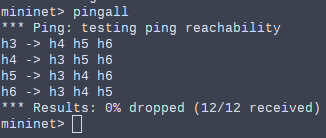
\includegraphics[width=0.5\linewidth]{img/task-7-step-2.png}
\end{figure}



\subsubsection*{Task 7 - Step 3}
\textit{Verify that the bandwidth and the delay of each link comply with the values
specified in the topology diagram shown in figure 1. Write in the lines below
the commands you used and the results you obtained.}

\begin{itemize}
  \item \code{h3 ping h4 -c 10}

  Output:
  \begin{lstlisting}
  --- 10.0.0.2 ping statistics ---
  5 packets transmitted, 5 received, 0% packet loss, time 4006ms
  rtt min/avg/max/mdev = 23.186/25.264/26.760/1.507 ms
  \end{lstlisting}
  The average RTT is approximately 20ms, wich comply the link delays values
  specified in the topology diagram. The same proceeding can be used to test the
  delay of all the others links.

  It's important to point out that the link delay between the two switches doesn't
  comply with the topology diagram: this behavior is however acceptable and it's due to
  the fact that in Mininet the switches are by default run in the same network
  namespace inside the kernel space, therefore they communicate to each other
  without using the link which has the performance parameters specified
  in the Python script.

  \item \code{iperf h3 h4}

  Output:
  \begin{lstlisting}
  *** Iperf: testing TCP bandwidth between h3 and h6
  *** Results: ['4.75 Mbits/sec', '6.23 Mbits/sec']
  \end{lstlisting}

  The same proceeding can be used to test the bandwidth between all nodes.
\end{itemize}



\subsubsection*{Task 8 - Question 1}
\textit{What are the advantages of having more controllers instead of
one single controller which serves all the switches of the network?}
\begin{itemize}
  \item \textbf{More performance}:  having more controllers makes each controller serve fewer
  nodes, therefore reducing its workload and improving the network performance.
  Moreover using more controllers makes it possible to choose where to position
  each controller: choosing a good placement increases the performance
  of the newtork by reducing the delay between each switch and the relative
  controller.
  \item \textbf{More fault tolerance}: the SDN controller is not a SPOF \footnote{SPOF = single point of failure}
  anymore because the network includes more controllers, so if one of the them
  fails the network can still work if there is at least another controller which can replace it.
  This can be achieved for example connecting each switch to multiple controllers
  or connecting the switches to a load balancer which acts like a ``man in the middle'' and
  forwards the requests that receives only to working controllers.
\end{itemize}


\subsubsection*{Task 8 - Question 2}
\textit{Would the fault tolerance of the network shown in figure \ref{fig:topology-1}
change if only one controller (linked to both the switches) was used
instead of two?}

No because in this topology each switch is connected only to a single controller,
therefore a failure of one of the two controllers prevents the network from
working properly, just like in the case of a single controller connected to both switches.





\subsubsection*{Task 8 - Question 3}
\textit{In this activity the topology shown in figure 1 was implemented
assuming that the two controllers were local controllers. How
would you have to change the Python script you created in this
activity in order to use remote controllers instead of local ones?
(Hint: see reference [5])}

The changes that has to be applied to the Python script are marked with the red
colour in the listing below.

\lstset{
 upquote=true,
 showspaces=false,
 showtabs=false,
 frame=single,
 tabsize=2,
 breaklines=true,
 numbers=left,
 showstringspaces=false,
 breakatwhitespace=true,
 escapeinside={(*@}{@*)},
 keywordstyle=\bfseries,
 basicstyle=\scriptsize\ttfamily,
 moredelim=**[is][\color{red}]{@}{@},
}
\begin{minipage}{\linewidth}
\begin{lstlisting}
#!/usr/bin/Python
from mininet.net import Mininet
from mininet.node import Controller, OVSSwitch, @RemoteController@
from mininet.cli import CLI
from mininet.log import setLogLevel, info
from mininet.link import TCLink

def multiControllerNet():
    net = Mininet( controller=Controller, switch=OVSSwitch, link=TCLink )

    info( "*** Creating hosts\n" )
    h1 = net.addHost('h3')
    h2 = net.addHost('h4')
    h3 = net.addHost('h5')
    h4 = net.addHost('h6')

    info( "*** Creating switches\n" )
    s1 = net.addSwitch( 's1' )
    s2 = net.addSwitch( 's2' )

    info( "*** Creating links\n" )
    net.addLink( h1, s1, bw=5, delay='5ms' )
    net.addLink( h2, s1, bw=5, delay='5ms' )
    net.addLink( h3, s2, bw=5, delay='5ms' )
    net.addLink( h4, s2, bw=5, delay='5ms' )
    net.addLink( s1, s2, bw=10, delay='2ms' )

    info( "*** Creating (reference) controllers\n" )
    c0 = net.addController( 'c0', @controller=RemoteController, ip='127.0.0.1'@, port=6633 )
    c1 = net.addController( 'c1', @controller=RemoteController, ip='127.0.0.1'@, port=6634 )

    info( "*** Starting network\n" )
    net.build()
    c0.start()
    c1.start()
    s1.start( [ c0 ] )
    s2.start( [ c1 ] )

    info( "*** Running CLI\n" )
    CLI( net )

    info( "*** Stopping network\n" )
    net.stop()

if __name__ == '__main__':
    setLogLevel( 'info' )
    multiControllerNet()
\end{lstlisting}
\end{minipage}
\lstset{
 upquote=true,
 showspaces=false,
 showtabs=false,
 frame=none,
 tabsize=2,
 breaklines=true,
 numbers=none,
 showstringspaces=false,
 breakatwhitespace=true,
 escapeinside={(*@}{@*)},
 keywordstyle=\bfseries,
 basicstyle=\scriptsize\ttfamily,
 moredelim=**[is][\color{red}]{@}{@},
}

For simplicity it has been assumed that the two remote controllers are running on the same machine on
which Mininet is running, therefore the ip \code{127.0.0.1} has been used (if the
controllers had been on different machines the relative IP should have been used).




\subsubsection*{Task 8 - Question 4}
\textit{How could we improve the fault tolerance of the network shown
in figure 1 making minor changes to the Python script used?}

The easiest way is to connect each switch to both the controllers, so that if
one controller fails the other one can still serve the switches keeping therefore
the network working. It is possible to do that simply modifying the lines 36 and 37 of
the Python script used in activity 1 (shown in listing \ref{lst:activity-1-script})
like this:

\begin{lstlisting}
s1.start( [ c0, c1 ] )
s2.start( [ c0, c1 ] )
\end{lstlisting}







\subsection*{Activity 2}
\subsubsection*{Task 5 - Step 2}
\textit{Test the created topology: verify the network connectivity between all hosts.
Write in the lines below the commands you used and the results you obtained.}
\begin{figure}[htb]
	\centering
	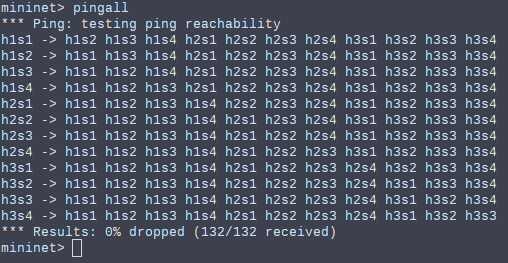
\includegraphics[width=0.8\linewidth]{img/activity-2-task-5-step-2.png}
\end{figure}


\subsubsection*{Task 5 - Step 3}
\textit{Verify the bandwidth and the delay between the hosts h1s1 and h3s4. Write
in the lines below the commands you used and the results you obtained.}
\begin{itemize}
  \item \code{iperf h1s1 h3s4}

  Result:
  \begin{lstlisting}
  *** Iperf: testing TCP bandwidth between h1s1 and h3s4
  *** Results: ['4.25 Gbits/sec', '4.26 Gbits/sec']
  \end{lstlisting}

  \item \code{h1s1 ping h3s4 -c 10}

  Result:
  \begin{lstlisting}
  --- 10.0.0.12 ping statistics ---
  10 packets transmitted, 10 received, 0% packet loss, time 9006ms
  rtt min/avg/max/mdev = 0.107/4.042/24.062/7.490 ms
  \end{lstlisting}
\end{itemize}




\subsubsection*{Task 6 - Question 1}
\textit{In this activity you implemented a network with multiple controllers using
a custom switch class and the high-level API. Which are the advantages of using
this method instead of the one used in Activity 1? What about the disadvantages?}

The advantage of the high level API is that it allows to write reusable code by
giving the possibly to create parametrized topology templates. Each template can
be used for easily creating different (and eventually complex) topologies based on it.

The main disadvantages are the higher complexity and the limitations in configuring
the networks nodes an links.
\subsubsection*{Task 6 - Question 2}
\textit{In this activity the topology shown in figure 2 was implemented
assuming that all the controllers were local controllers. How would
you have to change the Python script you created in this activity
in order to use remote controllers instead of local ones?}

It is necessary only to import the class \code{RemoteController} and modify the
lines 8,9,10,11 like this:

\begin{lstlisting}
c0 = RemoteController( 'c0', ip='127.0.0.1', port=6633 )
c1 = RemoteController( 'c1', ip='127.0.0.1', port=6634 )
c2 = RemoteController( 'c2', ip='127.0.0.1', port=6635 )
c3 = RemoteController( 'c3', ip='127.0.0.1', port=6636 )
\end{lstlisting}

Note that it has been assumed that the two remote controllers are running on the
same machine on which Mininet is running, therefore the ip \code{127.0.0.1} has
been used.


\subsubsection*{Task 6 - Question 3}
\textit{Try to modify the script you realized in order to have only
two controllers instead of four, each one linked to two different
switches. Each switch must be linked to a controller.}

The lines of code that has to be changed are showed in red in the script below.

\lstset{
 upquote=true,
 showspaces=false,
 showtabs=false,
 frame=single,
 tabsize=2,
 breaklines=true,
 numbers=left,
 showstringspaces=false,
 breakatwhitespace=true,
 escapeinside={(*@}{@*)},
 keywordstyle=\bfseries,
 basicstyle=\scriptsize\ttfamily,
 moredelim=**[is][\color{red}]{@}{@},
}
\begin{minipage}{\linewidth}
\begin{lstlisting}
#!/usr/bin/Python
from mininet.net import Mininet
from mininet.node import OVSSwitch, Controller
from mininet.topo import LinearTopo
from mininet.log import setLogLevel
from mininet.cli import CLI


@c0 = Controller( 'c0', port=6633 ) @
@c1 = Controller( 'c1', port=6634 ) @

@controllers = [c0, c1] @
@cmap = { 's1': c0, 's2': c0, 's3': c1, 's4' : c1 } @



class MultiSwitch( OVSSwitch ):
  def start( self, controllers ):
    return OVSSwitch.start( self, [ cmap[ self.name ] ] )


def multiControllerNet():
  topo = LinearTopo( k=4, n=3 )
  net = Mininet( topo=topo, switch=MultiSwitch, build=False)

  for c in controllers:
    net.addController(c)

  net.build()
  net.start()
  CLI( net )
  net.stop()

if __name__ == '__main__':
  setLogLevel( 'info' )
  multiControllerNet()
\end{lstlisting}
\end{minipage}






\subsection*{Challenge solution}
\subsubsection*{Task 1}
One possible solution to the task 1 is implementing the network using a Python
script and the Mininet middle-level API. The script is shown in the listing below.
\begin{lstlisting}
#!/usr/bin/Python
from mininet.net import Mininet
from mininet.node import Controller, RemoteController, OVSSwitch
from mininet.cli import CLI
from mininet.log import setLogLevel, info

def multiControllerNet():
    net = Mininet( controller=Controller, switch=OVSSwitch )

    info( "*** Creating hosts\n" )
    h1 = net.addHost('h1')
    h2 = net.addHost('h2')
    h3 = net.addHost('h3')
    h4 = net.addHost('h4')
    h5 = net.addHost('h5')
    h6 = net.addHost('h6')
    h7 = net.addHost('h7')
    h8 = net.addHost('h8')

    info( "*** Creating switches\n" )
    s1 = net.addSwitch( 's1' )
    s2 = net.addSwitch( 's2' )
    s3 = net.addSwitch( 's3' )
    s4 = net.addSwitch( 's4' )
    s5 = net.addSwitch( 's5' )
    s6 = net.addSwitch( 's6' )
    s7 = net.addSwitch( 's7' )

    info( "*** Creating links\n" )

    net.addLink( h1, s4 )
    net.addLink( h2, s4 )

    net.addLink( h3, s5 )
    net.addLink( h4, s5 )

    net.addLink( h5, s6 )
    net.addLink( h6, s6 )

    net.addLink( h7, s7 )
    net.addLink( h8, s7 )


    net.addLink( s4, s2 )
    net.addLink( s5, s2 )
    net.addLink( s6, s3 )
    net.addLink( s7, s3 )


    net.addLink( s2, s1 )
    net.addLink( s3, s1 )



    info( "*** Creating (reference) controllers\n" )
    c0 = net.addController( 'c0', controller=RemoteController, ip='127.0.0.1', port=6635 )
    c1 = net.addController( 'c1', controller=RemoteController, ip='127.0.0.1', port=6636 )
    c2 = net.addController( 'c2', port=6633 )
    c3 = net.addController( 'c3', port=6634 )


    info( "*** Starting network\n" )
    net.build()
    c0.start()
    c1.start()
    c2.start()
    c3.start()

    s1.start( [ c0, c1 ] )
    s2.start( [ c0, c1 ] )
    s3.start( [ c0, c1 ] )
    s4.start( [ c2 ] )
    s5.start( [ c2 ] )
    s6.start( [ c3 ] )
    s7.start( [ c3 ] )

    info( "*** Running CLI\n" )
    CLI( net )

    info( "*** Stopping network\n" )
    net.stop()

if __name__ == '__main__':
    setLogLevel( 'info' )
    multiControllerNet()
\end{lstlisting}
\lstset{
 upquote=true,
 showspaces=false,
 showtabs=false,
 frame=none,
 tabsize=2,
 breaklines=true,
 numbers=none,
 showstringspaces=false,
 breakatwhitespace=true,
 escapeinside={(*@}{@*)},
 keywordstyle=\bfseries,
 basicstyle=\scriptsize\ttfamily,
 moredelim=**[is][\color{red}]{@}{@},
}

\subsubsection*{Task 2}
These are the commands for connecting the switches served by \code{c3} to the controller
\code{c2}:
\begin{lstlisting}
sudo ovs-vsctl set-controller s6 tcp:127.0.0.1:6635
sudo ovs-vsctl set-controller s7 tcp:127.0.0.1:6635
\end{lstlisting}


\begin{thebibliography}{99}
  \footnotesize

  \bibitem{ref-7}
  Allouzi, M. (2015),
  \textit{Programming Assignment 2: Using Mininet and Mininet Python API: Instructions},
  lecture notes,
  Software defined networking Kent State University,
  Available at: {\scriptsize \url{http://www.cs.kent.edu/~mallouzi/Software%20Defined%20Networking/Assignment2.pdf}}

  \bibitem{ref-2}
  Blial, O., Ben Mamoun, M. and Benaini, R. (2016).
  An Overview on SDN Architectures with Multiple Controllers.
  \textit{Journal of Computer Networks and Communications}, pp.1-8.

  \bibitem{ref-1}
  Hai, N. and Kim, D. (2016).
  Efficient load balancing for multi-controller in SDN-based mission-critical networks.
  \textit{2016 IEEE 14th International Conference on Industrial Informatics (INDIN)}, pp.420-425

  \bibitem{ref-9}
  Phemius, K., Bouet, M. and Leguay, J. (2014).
  DISCO: Distributed SDN controllers in a multi-domain environment.
  \textit{2014 IEEE Network Operations and Management Symposium (NOMS)}.

  \bibitem{ref-4}
  GitHub. (n.d.).
  \textit{Introduction to Mininet}. [online].
  Available at: {\scriptsize \url{https://github.com/mininet/mininet/wiki/Introduction-to-Mininet#controllers}}
  [Accesed 3 Apr. 2018].

  \bibitem{ref-3}
  GitHub. (2016).
  \textit{mininet}. [online].
  Available at: {\scriptsize \url{https://github.com/mininet/mininet/blob/master/examples/controllers2.py}}
  [Accessed 28 Mar. 2018].

  \bibitem{ref-6}
  GitHub. (2016).
  \textit{mininet}. [online].
  Available at: {\scriptsize \url{https://github.com/mininet/mininet/blob/master/examples/controllers.py}}
  [Accessed 28 Mar. 2018].

  \bibitem{ref-8}
   Wiki.opendaylight.org. (n.d.).
   \textit{OpenDaylight OpenFlow Plugin::Mininet with multiple controllers}. [online].
   Available at: {\scriptsize \url{https://wiki.opendaylight.org/view/OpenDaylight_OpenFlow_Plugin::Mininet_with_multiple_controllers}}
   [Accessed 12 Apr. 2018].

  \bibitem{ref-5}
  GitHub. (2014).
  \textit{Reg:Mininet with multiple external Remote controllers - Issue \#319}. [online].
  Available at: {\scriptsize \url{https://github.com/mininet/mininet/issues/319}}
  [Accessed 30 Mar. 2018]
\end{thebibliography}

\end{document}
